\subsection{Real-time performance of the \pf{}}
\label{sec:pf_issues}



The two components of the model to assess are the iteration timings and the performance of the particle filter itself. That is, does the program run fast enough to be feasible in real-time, and is the model (and its \pf{} implementation) capable of modelling transit vehicles in real-time?


\paragraph{Is the particle filter fast enough?}
At peak hour on a typical weekday morning, there can be in excess of 1000~buses operating in Auckland. This leads to having more than $1000\Np$~particles in memory, each being mutated and reweighted approximately once every 30~seconds or so. By varying $N$, we can control how quickly each set of observations is processed. \Cref{fig:pf_timings} shows the average timings of the vehicle model component of our application, as well as the average time per particle, for varying $N$. More particles require more processing power, though there is additional overhead during the \emph{resampling} phase. Limiting the frequency of resampling is therefore necessary to make the program run faster, which is why we use the effective sample size, $\Neff$, described in \cref{eq:Neff} on \cpageref{eq:Neff}.


\begin{knitrout}\small
\definecolor{shadecolor}{rgb}{0.969, 0.969, 0.969}\color{fgcolor}\begin{figure}

{\centering 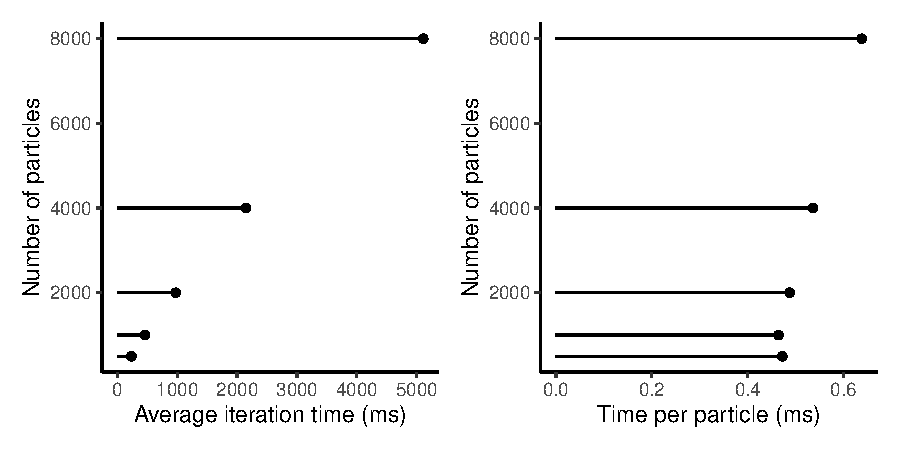
\includegraphics[width=.8\textwidth]{figure/pf_timings-1} 

}

\caption[Timings of the particle filter implemention for varying number of particles]{Timings of the particle filter implemention for varying number of particles. Left: the average iteration time (wall clock). Right: the average time per particle.}\label{fig:pf_timings}
\end{figure}


\end{knitrout}


\paragraph{How does the model perform?}





To assess how well our model performs in real-time, we repeated the simulation with a range of values of system noise $\Vnoise$, \gls{gps} error $\GPSerr$, and the number of particles $\Np$. For each simulation, we computed \emph{proportional effective sample size}, \emph{degeneration rate}, and \emph{relative variance}.

The \emph{proportional effective sample size} is the effective sample size relative to $N$, $\tilde N_\text{eff} = \frac{\Neff}{\Np}$. The higher this value, the less often the vehicle's state needs resampling, decreasing the average iteration time. \Cref{fig:model_performance_neff} shows the effect of $\Np$, system noise, and \gls{gps} error on $\tilde N_\text{eff}$. The most striking relationship is between $\tilde N_\text{eff}$ and \gls{gps} error: for larger error, more particles retain a high likelihood, and so the total weight is more evenly distributed. Conversely, larger values of system noise result in more variation between particles, leading to fewer particles ending near the observation position and decreasing $\tilde N_\text{eff}$.

\begin{knitrout}\small
\definecolor{shadecolor}{rgb}{0.969, 0.969, 0.969}\color{fgcolor}\begin{figure}

{\centering 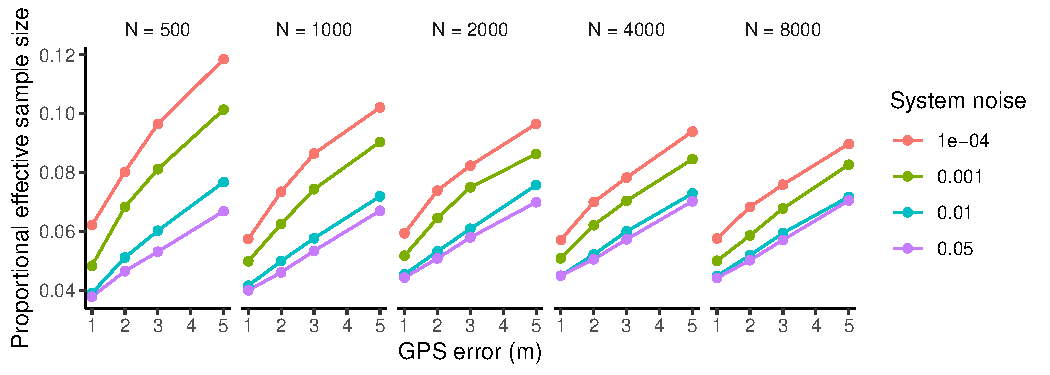
\includegraphics[width=\textwidth]{figure/model_performance_neff-1} 

}

\caption[Proportional effective sample size for varying values of GPS error, system noise, and number of particles]{Proportional effective sample size for varying values of GPS error, system noise, and number of particles.}\label{fig:model_performance_neff}
\end{figure}


\end{knitrout}


The \emph{degeneration rate} is the proportion of samples in which no particles end near the vehicle's reported position. In this case, all the particle likelihoods tend to zero, so the weights become undefined, resulting in the need to reinitialise the vehicle's state which results in the loss of any vehicle speed information along the most recently travelled road segment(s). We see from \cref{fig:model_performance_degen} that increasing \gls{gps} error or the number of particles reduces degeneration rate while increasing system noise shows a negligible reduction in degeneration rate. Larger \gls{gps} error means that particles do not need to end as close to the observed location to have a positive likelihood while increasing $\Np$ means more chance for a particle to end near the true bus.

\begin{knitrout}\small
\definecolor{shadecolor}{rgb}{0.969, 0.969, 0.969}\color{fgcolor}\begin{figure}

{\centering 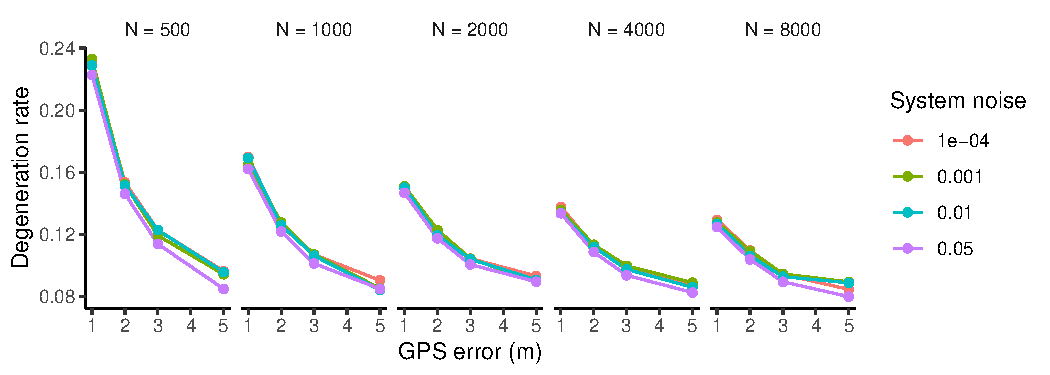
\includegraphics[width=\textwidth]{figure/model_performance_degen-1} 

}

\caption[Degeneration rate for varying values of GPS error, system noise, and number of particles]{Degeneration rate for varying values of GPS error, system noise, and number of particles.}\label{fig:model_performance_degen}
\end{figure}


\end{knitrout}

Finally, we have \emph{relative speed variance} along roads, which we use to compare the precision of the various models. It is the ratio of variance for a single simulation compared to the overall variance for all simulations. Let $\vec z_\ell^{e,s}$ be a vector of all vehicle speeds along road segment $\ell$ during the simulation with \gls{gps} error and system noise equal to $e$ and $s$, respectively. The ratio of the variance of speed for the single simulation compared to all simulations along one single road segment is given by
\begin{equation}
\label{eq:rel_speed_var_ratio}
v_\ell^{e,s} =
\frac{
    \mathrm{Var}(\vec z_\ell^{e,s})
}{
    \mathrm{Var}(\cup_e\cup_s \vec z_\ell^{e,s})
}.
\end{equation}
That is, for each segment in each simulation, we have a value representing whether this simulation estimates speed more or less accurately. We then compute the average ratio for all $L$ road segments,
\begin{equation}
\label{eq:rel_speed_var}
\bar v^{e,s} = \frac{1}{L} \sum_{\ell=1}^L v_\ell^{e,s}.
\end{equation}
A small value of $\bar v^{e,s}$ tells us that, on average, the simulation with \gls{gps} error $e$ and system noise $s$ estimates road speed \emph{with greater precision} than the other simulations. \Cref{fig:model_performance_var} presents these results, where we see the greatest effect on relative variance caused by increasing \gls{gps} error. Increasing $\Np$ produces a small decrease, and changes to system noise show no discernible effect.


\begin{knitrout}\small
\definecolor{shadecolor}{rgb}{0.969, 0.969, 0.969}\color{fgcolor}\begin{figure}

{\centering 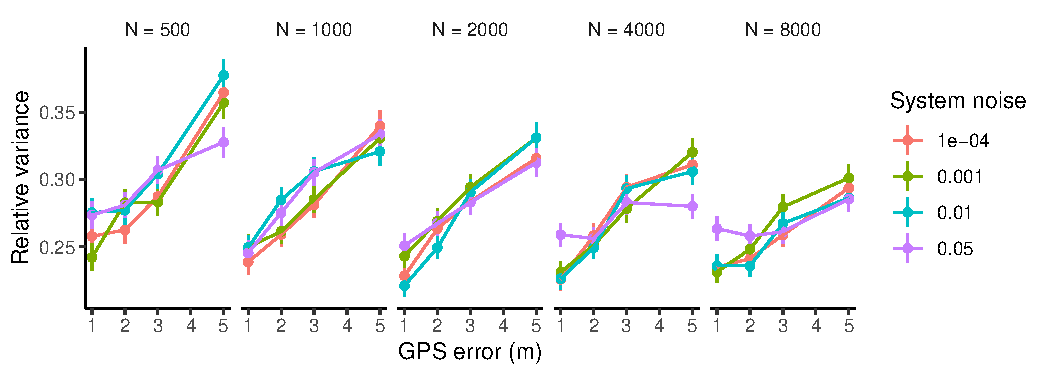
\includegraphics[width=\textwidth]{figure/model_performance_var-1} 

}

\caption[Relative speed variance for varying values of GPS error, system noise, and number of particles]{Relative speed variance for varying values of GPS error, system noise, and number of particles.}\label{fig:model_performance_var}
\end{figure}


\end{knitrout}


The results displayed in \cref{fig:model_performance_neff,fig:model_performance_degen,fig:model_performance_var} present a \emph{trade-off} between performance and estimation. Increasing \gls{gps} error increases the effective sample size, which reduces the frequency of resampling and speeds up each iteration. We also see a reduction in the rate of degeneration, which implies the particle filter is less likely to lose the vehicle and provide the desired speed estimates. However, increasing \gls{gps} error also increases the relative uncertainty of speed estimates. Increasing the number of particles generally results in a reduction in both degeneration rate and relative uncertainty, but, from \cref{fig:pf_timings}, this comes at the cost of increased computational demand.
